\pagebreak
\subsection{Tecnologie di supporto allo sviluppo}
\label{sez:tecnologie-supporto-sviluppo}


\subsubsection{\gls{npm}}

\gls{npm} è il gestore ufficiale dei pacchetti per \textit{Node.js}, utilizzato per installare, condividere e gestire librerie e moduli \textit{JavaScript}.\\
Grazie a \gls{npm}, gli sviluppatori possono facilmente configurare e gestire le dipendenze necessarie per il proprio progetto, semplificando notevolmente il flusso di lavoro.\\

\noindent Nel contesto del mio progetto, ho utilizzato \gls{npm} per gestire le dipendenze sia del \gls{frontend} che del \gls{backend}.\\
Per il \gls{frontend}, ha permesso di installare librerie come \textit{React}, \textit{Material-UI} ed altre dipendenze necessarie per lo sviluppo dell'interfaccia utente. \\
Per il \gls{backend}, \gls{npm} ha facilitato l'installazione di pacchetti come \textit{NestJS}, \textit{Mongoose} e altre librerie essenziali per la gestione delle \gls{api} e la comunicazione con il database \textit{MongoDB}. \\

\noindent Utilizzando \gls{npm}, è stato possibile garantire che tutte le dipendenze fossero correttamente gestite e aggiornate, migliorando così l'efficienza e la manutenibilità del progetto.

\subsubsection{Docker}

\noindent Docker è una piattaforma che consente di creare, distribuire e gestire applicazioni tramite \gls{container} leggeri e portatili.\\

\noindent I \gls{container} consentono di isolare le applicazioni e le loro dipendenze, garantendo che l'ambiente di esecuzione sia consistente e riproducibile su qualsiasi sistema, che si tratti di sviluppo, \textit{test} o produzione.\\
Questa tecnologia semplifica notevolmente il processo di \textit{deployment}, risolvendo i problemi di compatibilità tra ambienti diversi. \\
I \gls{container} offrono anche un'esecuzione più veloce e scalabile delle applicazioni.\\

\noindent Nel progetto ho utilizzato \textit{Docker} per eseguire un'istanza di \textit{MongoDB} in un \gls{container}.\\
Questo approccio ha consentito di configurare facilmente un ambiente di \textit{database} locale per lo sviluppo, mantenendo la stessa configurazione e versioni di \textit{MongoDB} tra i vari ambienti, come quelli di \textit{test} e produzione.\\
Grazie a \textit{Docker}, è stato possibile isolare \textit{MongoDB} dal resto dell'applicazione, semplificando la gestione delle dipendenze e facilitando il processo di \textit{deployment} in ambienti diversi.

\subsubsection{Postman}

\textit{Postman} è uno strumento potente e intuitivo che consente di testare facilmente le \gls{api}.\\
Permette di inviare richieste \gls{http}, come \texttt{GET}, \texttt{POST}, \texttt{PUT} e \texttt{DELETE}, e analizzare le risposte ricevute, semplificando notevolmente il processo di sviluppo e \textit{debugging} delle \gls{api}.\\
Grazie alla sua interfaccia grafica, \textit{Postman} offre un modo semplice per definire i parametri delle richieste, visualizzare i risultati e monitorare il comportamento delle \gls{api} in tempo reale.\\

\noindent Nel progetto ho utilizzato \textit{Postman} durante la fase di codifica delle \gls{api} per facilitare il \textit{testing} delle varie funzionalità.\\
In particolare, è stato utilizzato per testare le \gls{api} di creazione e gestione dei progetti, inviando richieste con i parametri appropriati e verificando che le risposte fossero corrette e conformi alle specifiche.\\ 
Questo approccio ha permesso di identificare rapidamente eventuali errori o problemi di funzionamento, migliorando l'affidabilità e la qualità delle \gls{api} prima della loro integrazione nell'applicazione finale.\\

\noindent Nella {\hyperref[fig:postman]{Figura 1.8}} è possibile vedere un esempio di utilizzo di \textit{Postman} per testare una chiamata \gls{api}, in particolare quella di generazione di un progetto.

\begin{figure}[H]
    \label{fig:postman}
    \centering
    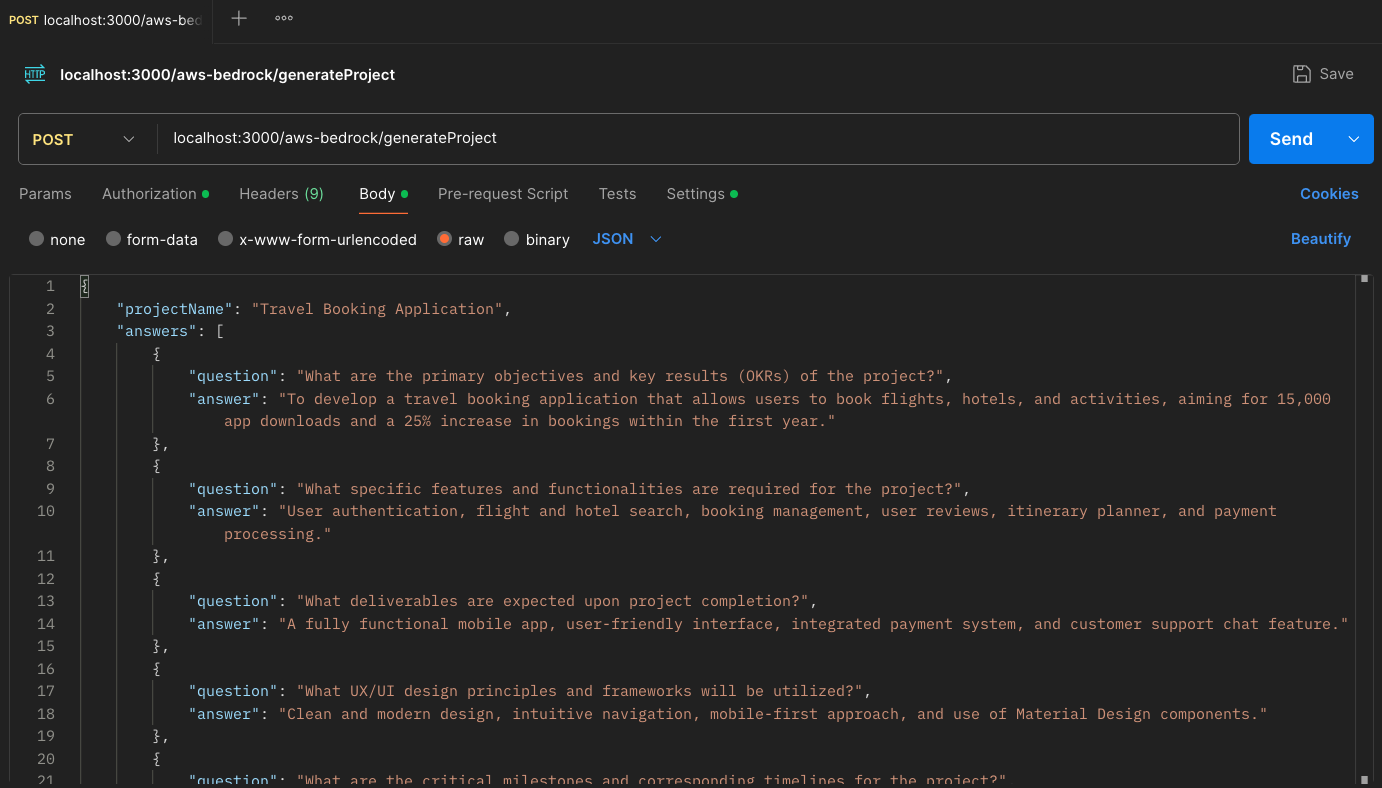
\includegraphics[scale=0.3]{tecnologie/postman.png}
    \caption{Esempio di utilizzo di \textit{Postman} per chiamata \gls{api}}
\end{figure}

\subsubsection{StarUML}

\textit{StarUML} è uno strumento avanzato per la modellazione di diagrammi \gls{uml}, un linguaggio standardizzato utilizzato per rappresentare visivamente le diverse componenti e interazioni di un sistema software. \\
\gls{uml} fornisce un set di diagrammi che permettono di descrivere vari aspetti di un sistema,
tra cui la struttura statica (come classi e oggetti) ed il comportamento dinamico (come interazioni e flussi di attività). \\
Tra i diagrammi \gls{uml} più utilizzati ci sono i diagrammi dei casi d'uso, di sequenza e delle attività, che sono fondamentali per la progettazione e la documentazione di applicazioni.\\

\noindent Nel progetto ho utilizzato \textit{StarUML} per creare i diagrammi dei casi d'uso, che rappresentano le interazioni tra gli attori (come gli utenti o i sistemi esterni) ed il sistema.\\
Questi diagrammi sono cruciali per descrivere le funzionalità offerte dal sistema e per evidenziare i vari scenari d'uso, facilitando la comprensione delle esigenze del progetto.\\
I diagrammi dei casi d'uso creati con \textit{StarUML} hanno semplificato la visualizzazione dei flussi operativi del sistema, migliorando la comunicazione tra il team di sviluppo e i clienti.

\subsubsection{Git}

\textit{Git} è un sistema di controllo di versione distribuito progettato per tracciare le modifiche al codice sorgente e facilitare la collaborazione tra sviluppatori, rendendo la gestione di progetti \textit{software} più efficiente e sicura.\\
Grazie alla sua natura distribuita, \textit{Git} permette ad ogni sviluppatore di lavorare in modo indipendente, mantenendo una copia completa del progetto sul proprio ambiente locale, e successivamente sincronizzare le modifiche con un \textit{repository} remoto.\\

\noindent Nel progetto ho utilizzato \textit{Git} per versionare l'intero codice, garantendo che ogni modifica fosse tracciata e documentata. \\
È stato essenziale per la gestione delle diverse versioni del progetto, permettendo di lavorare su funzionalità parallele attraverso l'uso dei \gls{branch}, e integrando le modifiche in modo sicuro tramite \gls{pr}. \\
In questo modo, è stato possibile mantenere un flusso di lavoro ordinato e privo di conflitti, garantendo che il codice rimanesse sempre aggiornato e facilmente recuperabile in caso di necessità. 

\subsubsection{MongoDB Compass}

\textit{MongoDB Compass} è un'interfaccia grafica intuitiva che facilita l'interazione con il \textit{database MongoDB}, permettendo di esplorare e modificare facilmente i dati, visualizzare gli indici, eseguire \textit{query}, e gestire il database in modo efficiente.\\
Grazie alla sua interfaccia visiva, semplifica operazioni complesse come la gestione della struttura dei dati, l'analisi delle prestazioni delle \textit{query}, e la visualizzazione dei documenti.\\

\noindent Nel progetto ho utilizzato \textit{MongoDB Compass}  per accedere facilmente al database \textit{MongoDB}, consentendo di visualizzare, modificare e analizzare i dati durante la fase di sviluppo.\\
È stato uno strumento fondamentale per esplorare le collezioni, controllare i dati inseriti, semplificando il processo di \textit{debugging} e ottimizzazione delle \textit{query}.\\
In questo modo, è stato possibile gestire e monitorare il \textit{database} con maggiore efficienza, garantendo un flusso di lavoro più rapido e preciso.\\

\noindent Nella {\hyperref[fig:mongodb-compass]{Figura 1.9}} è possibile vedere un esempio di utilizzo di \textit{MongoDB Compass} per visualizzare un documento all'interno di una collezione.

\begin{figure}[H]
    \label{fig:mongodb-compass}
    \centering
    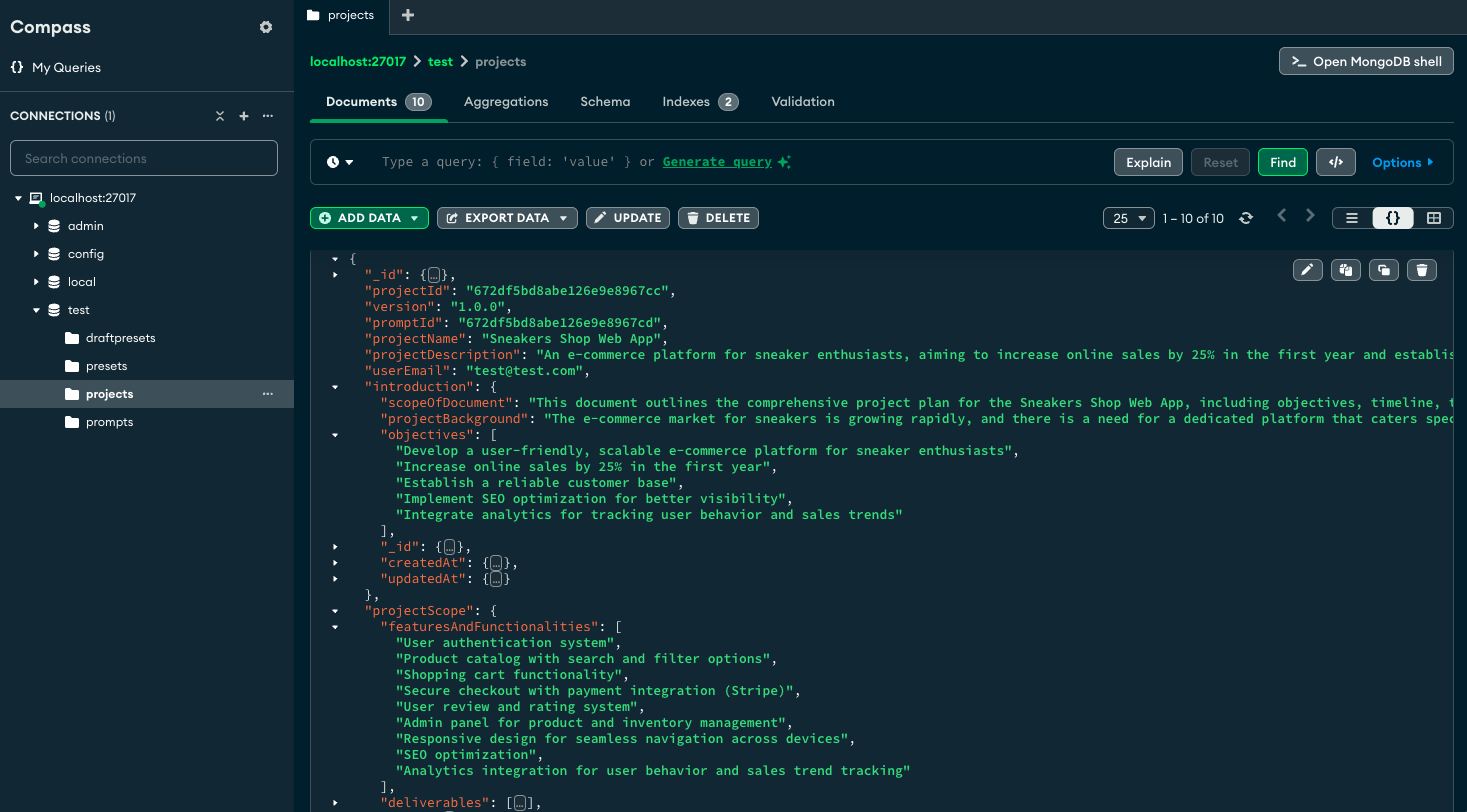
\includegraphics[scale=0.3]{tecnologie/mongodb-compass.png}
    \caption{Visualizzazione di un documento in \textit{MongoDB Compass}}
\end{figure}
